%
%

\chapter{国内外电动汽车充电系统标准综述}


\href{https://mp.weixin.qq.com/s/65C5toQG0SfH1YHTb1oKKw}{国内外电动汽车充电系统标准综述}

电动汽车是节能环保型车辆,由于对环境影响相对较小,其前景被广泛看好。但发展初期,各国对未来市场的发展没有统一的认识,且各国配电网络的电压频率等电气特性存在较大差异,故在制定标准上有所区别。标准的差异既造成了后续全球充电接口不统一、通信协议不兼容的现状,也引出了目前迫切融合的需求。

本文介绍了国内外电动汽车充电系统标准化的现状,主要从充电系统一般要求、充电接口、交流充电控制导引、直流充电通信协议等方面阐述了国内外技术方案的共性与差异,并对后续充电系统标准的融合及发展规划做了展望。


\section{电动汽车充电系统标准概述}
     
全球范围内电动汽车充电系统标准,主要有国际电工委员会(Intermnational Electro technical Commission,IEC)标准、欧洲电工标准化委员会(European Norm,EN)标准、美国汽车工程师协会(Society of Automotive Engineers,SAE)标准、日本电动汽车协会(CHArge de Move,CHAdeMO)标准以及我国GB/T标准。


\begin{table}[!htbp]
    \centering
    \renewcommand{\arraystretch}{1.5}
    \caption{国内外电动主要传导式充电系统标准}   
    \begin{tabular}{c|c|c|c|c|c|c}
        \specialrule{0.2em}{0pt}{0pt} 
        \multicolumn{2}{c|}{类别} & IEC标准 & EN标准 & SAE标准 & GB/T标准 & CHAdeMO标准\\
        \hline
        \multicolumn{2}{c|}{传导充电系统一般要求} & \textcolor{red}{\bf IEC 61851-1} & EN61851-1 & & \textcolor{red}{\bf GB/T18487.1——2015} & -\\
        \hline
        \multirow{3}{*}{充电连\newline 接装置}     & 一般要求  & IEC 62196-1   & EN 62196-1    &                            &GB/T20234.1——2015  &-  \\
                                                 & 交流接口  & IEC 62196-2   &EN 62196-2      & \textcolor{red}{\bf SAEJ1772}    &GB/T20234.2——2015  &-\\
                                                 & 直流接口 & IEC 62196-3   &EN 62196-3       &                            &GB/T20234.3——2015  &-\\
        \hline
        \multicolumn{2}{c|}{直流充电充电协议}        & IEC 61851-24 & EN61851-24 & & GB/T27930-2015 & CHAdeMO 3.0\\
        \specialrule{0.2em}{0pt}{0pt} 
    \end{tabular} 
\end{table}

\section{三个信号的关系}

在电动汽车(EV)充电系统中,CC(Connection Confirmation)、CP(Control Pilot)、和PP(Proximity Pilot)是关键的信号,它们共同确保充电过程的安全性和正确性。以下是这三个信号之间的关系及其各自的功能:

1. PP(Proximity Pilot)
功能:PP信号主要用于检测充电枪的物理状态,即充电插头的插入深度和连接情况。PP信号通过在插头和插座之间的物理连接来检测接近状态。
作用:
确认充电枪是否插入到位。
防止在插头未完全插入的情况下启动充电。
确定充电电缆的额定电流上限,以便限制通过充电线缆的最大电流,避免电缆过载。

2. CP(Control Pilot)
功能:CP信号是充电过程中的主要控制信号,负责在车辆与充电桩之间传递控制信息。通过PWM(脉冲宽度调制)信号来调节和传达信息。
作用:
确认车辆已连接并准备接收电流。
通知车辆和充电桩之间的通信状态。
控制充电过程的启动与停止,确保充电过程仅在安全状态下进行。
通过PWM信号调节充电电流的大小,基于车辆需求调整电流输出。

3. CC(Connection Confirmation)
功能:CC信号负责最终确认连接的整体安全性,并在充电开始前完成所有必要的检查。它通常依赖于CP和PP信号提供的信息,以确定是否可以安全地开始充电。
作用:
确认PP信号的接近检测状态,以及CP信号的通信和控制状态。
在确认连接安全、无误后,允许充电电流传输。
如果在充电过程中发现任何异常情况,CC信号将触发充电中断。

\noindent\textcolor{red}{\bf 信号关系}

PP → CC: PP信号首先检测插头的物理连接状态(如插入深度、锁定情况),确保物理连接已准备就绪。PP信号直接影响CC,因为如果PP检测到连接不当,CC不会允许充电过程启动。

CP → CC: CP信号用于控制充电过程,包括启动和停止充电。CP信号还包括与车辆通信的信息交换。CC利用CP信号的信息来进一步确认连接的电气状态。如果CP信号正常,CC信号会允许充电过程的继续。

CC作为最终确认:CC信号综合了PP和CP信号的信息,最终决定是否可以开始充电,确保在安全条件下进行充电。
总结来说,PP信号主要处理物理连接,CP信号处理充电控制和通信,而CC信号则是综合以上两者的信息,用于最终确认连接的安全性,确保充电过程能够安全进行。


\section{部分整理内容}
    \begin{enumerate}
        \item  CP信号的作用
            \begin{enumerate}
                \item  控制与通信:CP导线传递的是一个脉宽调制(PWM)信号,该信号由充电桩生成并发送给车辆。PWM信号的占空比直接决定了最大允许的充电电流。具体来说,占空比越高,表示允许的电流越大。车辆根据CP信号的占空比,调整其车载充电机(OBC)的充电电流。
            \end{enumerate}
        \item  CC导线的作用
            \begin{enumerate}
                \item 连接确认与电流限值:CC导线连接到充电插头内的一个电阻,通过检测这个电阻值,车辆和充电桩可以确认充电枪是否正确插入,并确定允许的最大充电电流。不同的电阻值代表不同的充电电缆或充电枪规格,这实际上限制了通过该电缆或充电枪的最大电流,防止过载或过热。  
            \end{enumerate}
        \item CP信号和CC电阻的综合判断
            \begin{enumerate}
                \item CP信号:告诉车辆和充电桩当前可使用的最大电流。
                \item CC电阻:提供物理电缆或充电枪的最大电流容量限制。
                \item 优先级机制:在实际应用中,CC电阻的限流机制通常是最高优先级的。如果CC电阻表明电缆只支持较小的电流,那么即使CP信号允许更大的电流,系统也会优先遵循CC导线的限流判断。
            \end{enumerate}
    \end{enumerate}

    \begin{figure}[!htbp]
        \centering
        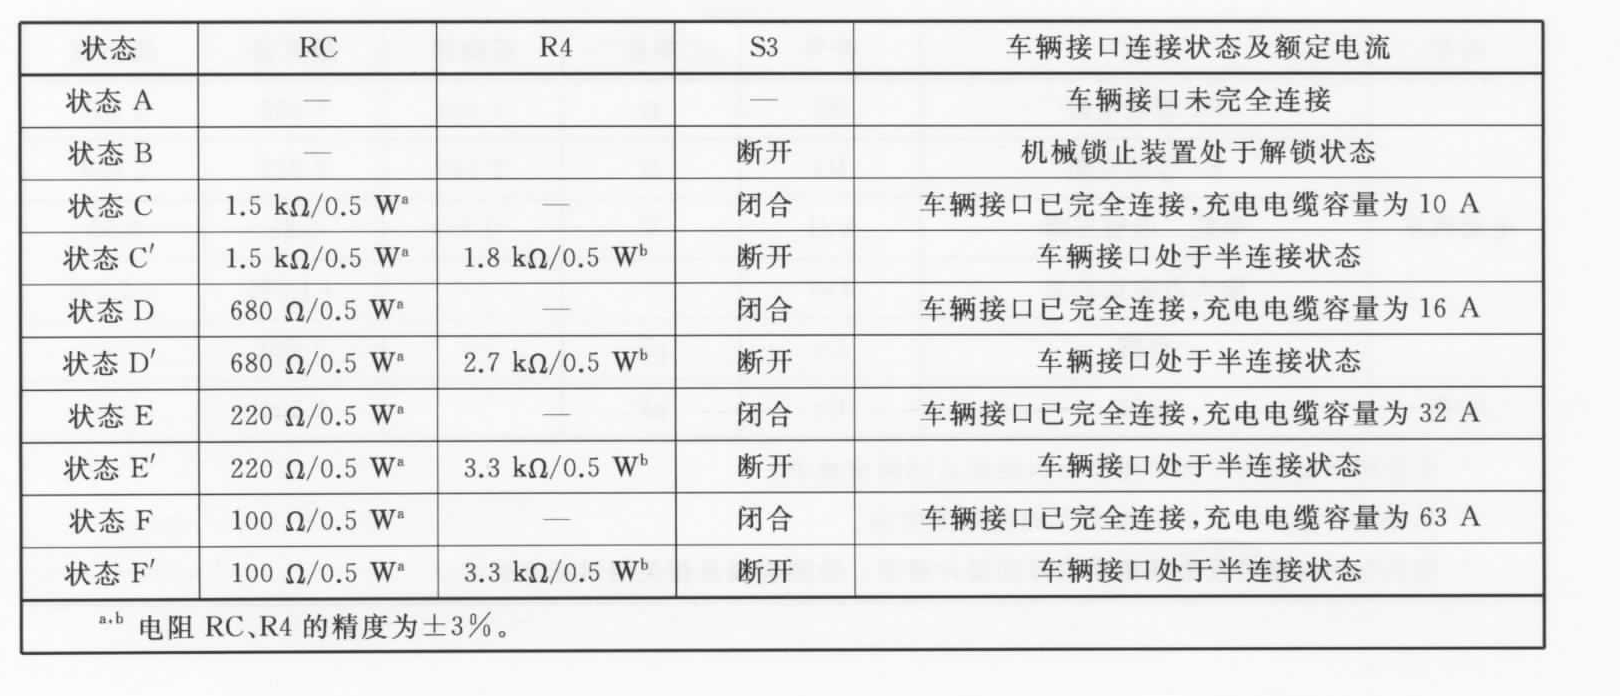
\includegraphics[width = 0.82\textwidth]{C11}
        \caption{车辆接口连接状态及Rc阻值\cite{GB18487_1}}
        \label{fig:C11}
    \end{figure}

